\documentclass[10pt, a4paper]{article}
\usepackage{enumerate, listings, enumitem, etoolbox}
\usepackage[spanish]{babel}
%\usepackage{a4wide} % márgenes un poco más anchos que lo usual
\usepackage{fullpage}
\usepackage[utf8]{inputenc}
\usepackage{aed2-symb,aed2-itef,aed2-tad,aed2-diseno}
\usepackage{color} % para snipets de codigo coloreados
\usepackage{fancybox}  % para el sbox de los snipets de codigo
\usepackage[paper=a4paper, left=1.5cm, right=1.5cm, bottom=1.5cm, top=3.5cm]{geometry}
\usepackage[utf8]{inputenc}
\usepackage[T1]{fontenc}
\usepackage[spanish]{babel}
\usepackage{indentfirst}
\usepackage{fancyhdr}
\usepackage{latexsym}
\usepackage{lastpage}
\usepackage[colorlinks=true, linkcolor=blue]{hyperref}
\usepackage{calc}
\usepackage{algorithmicx, algorithm}
\usepackage[noend]{algpseudocode}
\usepackage{xcolor}
\usepackage{enumerate, listings, enumitem, etoolbox}
\usepackage{pdfpages}

\newcommand{\bigO}{\mathcal{O}}
\newcommand{\asignar}[2]{$#1 \gets #2$}
\algrenewcommand\alglinenumber[1]{\tiny #1:}  % Para que los numeros de linea del pseudo sean pequeños
\renewcommand{\thealgorithm}{}  % Que no aparezca el numero luego de "Algorithm"
\floatname{algorithm}{ }    % Entre {  } que quiero que aparezca en vez de "Algorithm"

\parskip=5pt % 10pt es el tamaño de fuente
\parindent=0pt

\begin{document}

\thispagestyle{empty}
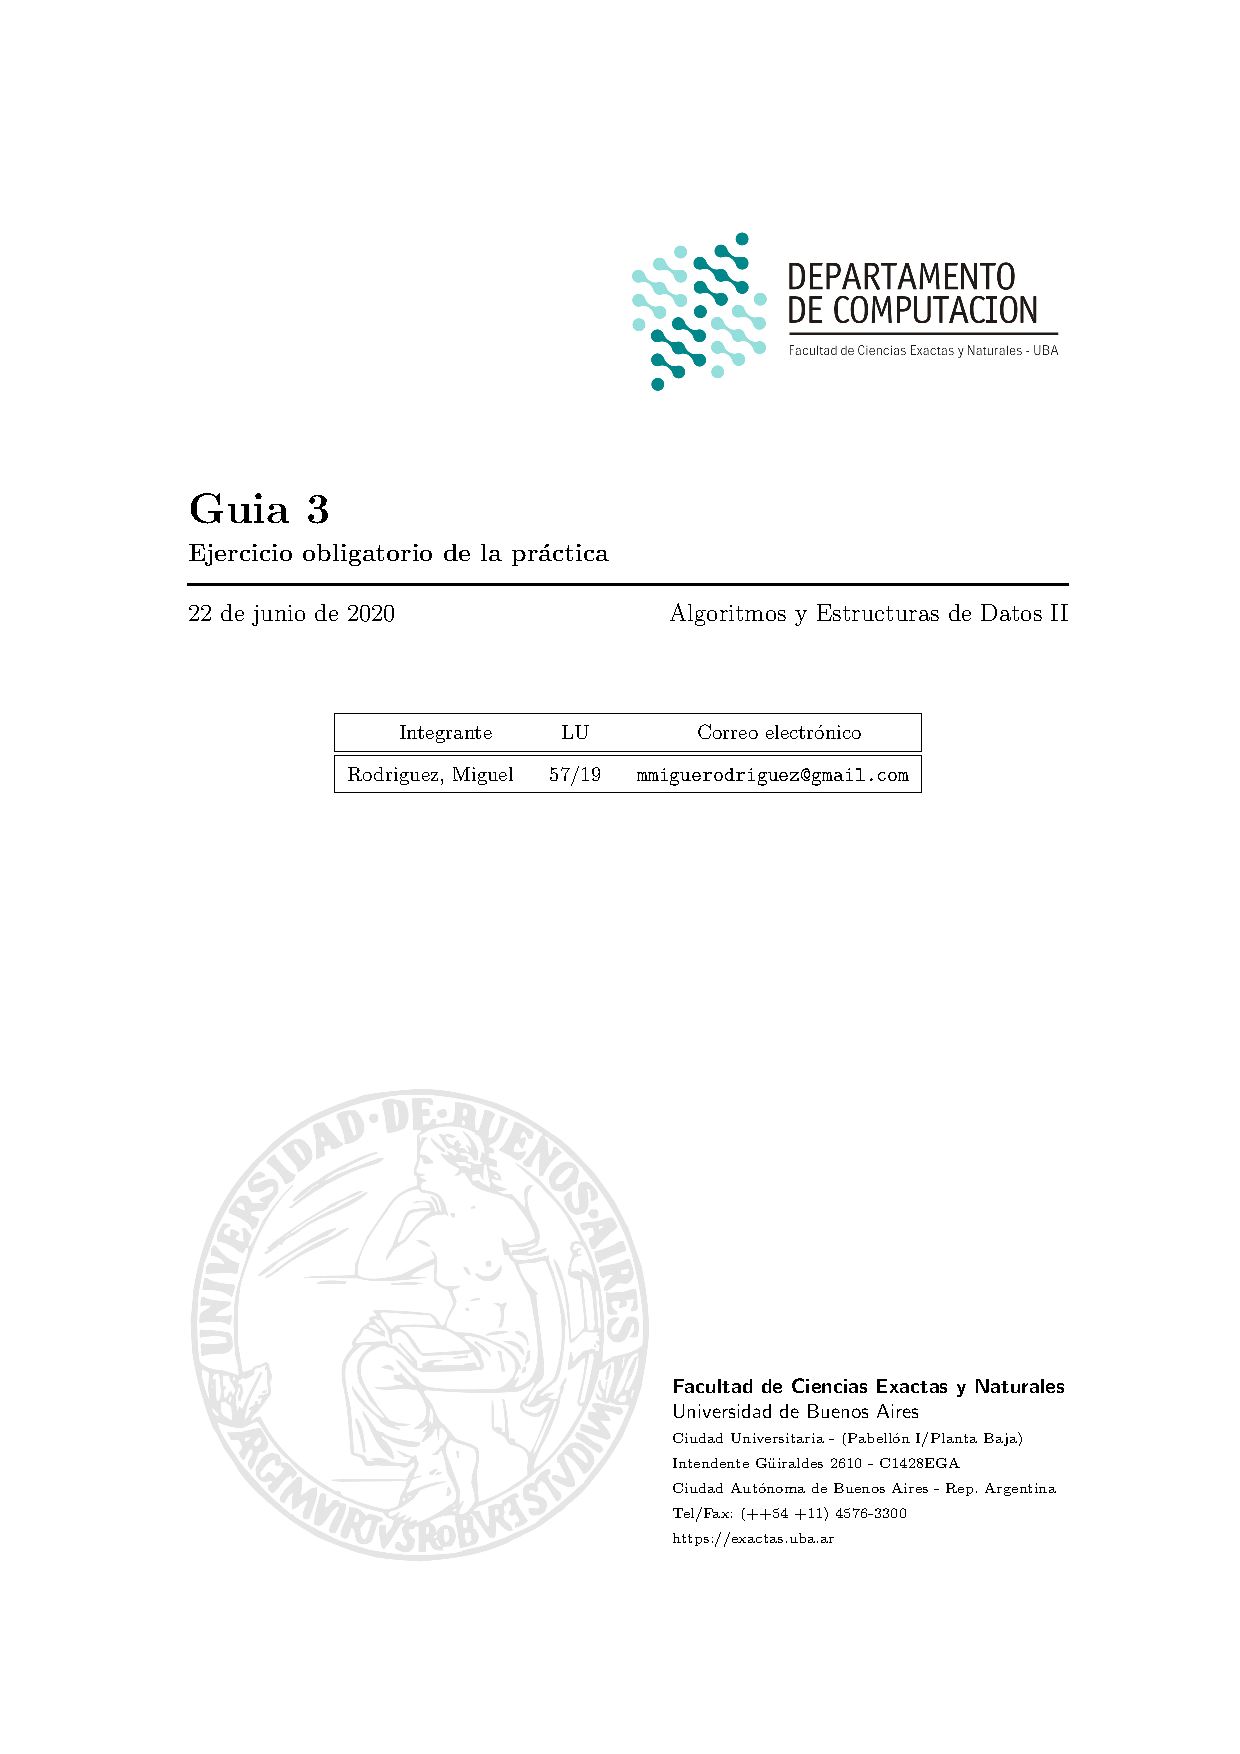
\includepdf[pages=-,pagecommand={},width=\textwidth]{caratula.pdf}

\setcounter{page}{1}
\section{Módulo Cumplea\~nos}

\begin{Interfaz}
  \textbf{se explica con}: \tadNombre{Cumplea\~nos}

  \textbf{géneros}: \TipoVariable{cumple}

  \Titulo{Operaciones básicas}

	\begin{enumerate}
	\item \TipoFuncion{publicarLista}{\Inout{c}{cumple}, \In{n}{negocio}, \In{\ell}{dicc(regalo, nat)}}{}
	\\\textbf{Complejidad:} $\bigO(L + log(N))$. L = \#claves($\ell$) y N = \#negocios(c).
	\item \TipoFuncion{regalos}{\In{c}{cumple}, \In{n}{negocio}}{conj(regalo)}
	\\\textbf{Complejidad:} $\bigO(log(N))$. N = \#negocios(c).
	\item \TipoFuncion{negociosConRegalos}{\In{c}{cumple}}{conj(negocio)}
	\\\textbf{Complejidad:} $\bigO(1)$.
	\item \TipoFuncion{regaloM\'asBarato}{\In{c}{cumple}}{regalo}
	\\\textbf{Complejidad:} $\bigO(1)$.
	\item \TipoFuncion{comprarRegaloM\'asBarato}{\Inout{c}{cumple}, \In{n}{negocio}, \In{l}{dicc(regalo, nat)}}{}
	\\\textbf{Complejidad:} $\bigO(N + log(R))$. N = \#negocios(c) y R = total regalos del sistema.
	\end{enumerate}
\end{Interfaz}

\begin{Representacion}
	\\ \TipoVariable{negocio} \textbf{es} \TipoVariable{nat} \\
	\TipoVariable{regalo} \textbf{es} \TipoVariable{nat} \\
	\TipoVariable{precio} \textbf{es} \TipoVariable{nat}
  \begin{Estructura}{cumple}[estr]
    \begin{Tupla}[estr]
      \tupItem{negocios}{diccAVL<negocio, minHeap$\langle$precio, itConj$\rangle$>}
      \tupItem{\\regalosPorNegocio}{diccAVL<negocio, conjLineal(regalo)>}
			\tupItem{\\negociosConRegalos}{conjAVL(negocio)}
			\tupItem{\\regaloM\'asBarato}{tupla<negocio, precio, itConj>}
    \end{Tupla}
  \end{Estructura}
\end{Representacion}

\begin{Algoritmos}
	\begin{enumerate}
		\item \TipoFuncion{publicarLista}{\Inout{c}{cumple}, \In{n}{negocio}, \In{\ell}{dicc(regalo, nat)}}{}
		\begin{enumerate}
			\item Itero sobre el diccionario de regalos y me armo dos conjuntos que no van a tener elementos repetidos, por esto, usamos \texttt{AgregarRapido()}. Uno de los conjuntos va a ser usado para guardar los regalos por negocio y otro va a ser usado para lo mismo, pero de forma ordenada por precio en un heap. Por cada elemento que inserto en el primer conjunto, guardo su iterador en el segundo conjunto y adem\'as, comparo el precio de cada regalo con el que tengamos en \texttt{c.regaloM\'asBarato}. En el que caso haya un nuevo regalo m\'as barato, lo reemplazamos (modificamos \texttt{c.regaloM\'asBarato} y le insertamos el nuevo negocio, precio e iterador al regalo). Costo: $\bigO(L)$. Iterar un conjunto. Generar dos conjuntos nuevos, sabiendo que no contienen repetidos.
			\item A partir del conjunto generado anteriormente que contenga por cada regalo su <precio, itConj>, uso BuildMinHeap para hacerme un heap que ordene a partir del precio del regalo y guarde su iterador para poder eliminar de \texttt{c.regalosPorNegocio} a futuro. Costo: $\bigO(L)$. Algoritmo de Floyd para generar un minHeap usando \textsc{Build-Min-Heap} y \textsc{Min-Heapify}\footnote{Cormen, \textit{Introduction To Algorithms (Third Edition)}, 156-159}.
			\item Inserto en \texttt{c.negociosConRegalos} el identificador del negocio. Costo: $\bigO(log(N))$. Inserci\'on en conjAVL.
			\item Inserto en \texttt{c.regalosPorNegocio} del negocio correspondiente el conjunto de regalos previamente generado. Costo: $\bigO(log(N))$. Definir en diccAVL.

			\begin{minipage}{\linewidth}
				\begin{algorithm}[H]
					\caption{\textbf{iPublicarLista}(\Inout{c}{cumple}, \In{n}{negocio}, \In{\ell}{dicc(regalo, nat)})}
					\begin{algorithmic}[1]
							\State \asignar{regalosPorNegocio}{Vacio()}
							\State \asignar{preciosIterador}{Vacio()}
							\State \asignar{itRegalos}{CrearIt(\ell)}
							\While{$HaySiguiente?(itRegalos)$} \Comment{$\bigO$(L)}
								\State \asignar{regalo}{SiguienteClave(itRegalos)}
								\State \asignar{precio}{SiguienteSignificado(itRegalos)}
								\State \asignar{itRegalo}{AgregarRapido(regalosPorNegocio, regalo)} \Comment{$\bigO$(1)}
								\State \asignar{heapElem}{\langle precio, itRegalo\rangle}
								\State $AgregarRapido(preciosIterador, heapElem)$ \Comment{$\bigO$(1)}
								\If{$precio < \pi_2(c.regaloMasBarato) \lor \pi_2(c.regaloMasBarato) = 0$}
									\State \asignar{c.regaloMasBarato}{\langle n, precio, itRegalo\rangle} \Comment{$\bigO$(1)}
								\EndIf
								\State $Avanzar(itRegalos)$
							\EndWhile
							\State \asignar{minHeap}{BuildMinHeap(preciosIterador)} \Comment{$\bigO$(L)}
							\State $Definir(c.negocios, n, minHeap)$ \Comment{$\bigO$(log(N))}
							\State $Definir(c.regalosPorNegocio, n, regalosPorNegocio)$ \Comment{$\bigO$(log(N))}
							\State $Agregar(c.negociosConRegalos, n)$ \Comment{$\bigO$(log(N))}
							\medskip
					\end{algorithmic}
				\end{algorithm}
			\end{minipage}
		\end{enumerate}

		\item \TipoFuncion{regalos}{\In{c}{cumple}, \In{n}{negocio}}{conj(regalo)}
		\begin{enumerate}
			\item Devolver el valor que se encuentra al \texttt{obtener(n, c.regalosPorNegocio)}. Costo: $\bigO(log(N))$. B\'usqueda en un diccAVL.
		\end{enumerate}

		\item \TipoFuncion{negociosConRegalos}{\In{c}{cumple}}{conj(negocio)}
		\begin{enumerate}
			\item Devolver el valor que se encuentra en \texttt{c.negociosConRegalos}. Costo: $\bigO(1)$. B\'usqueda en memoria.
		\end{enumerate}

		\item \TipoFuncion{regaloM\'asBarato}{\In{c}{cumple}}{regalo}
		\begin{enumerate}
			\item Devolver el valor que se encuentra en $Siguiente(\pi_{3}($\texttt{c.regaloM\'asBarato}$))$. Costo: $\bigO(1)$. B\'usqueda en memoria.
		\end{enumerate}

		\item \TipoFuncion{comprarRegaloM\'asBarato}{\Inout{c}{cumple}}{}
		\begin{enumerate}
			\item Buscar en \texttt{c.negocios} el minHeap en donde est\'a el regalo m\'as barato y extraerlo. Costo: $\bigO(log(N)$ + $log(R))$. B\'usqueda en diccABL + extraer el primer elemento y mantener ordenado un minHeap. El peor caso para extraer del minHeap con regalos es $log(R)$ y ocurre cuando un negocio contiene todos los regalos. El caso exacto es $log(regalos(negocio))$.
			\item En el caso que el negocio no tenga mas regalos, eliminar de la lista \texttt{c.negociosConRegalos} el negocio donde estaba el regalo m\'as barato. Costo: $\bigO(log(N))$. Eliminar en conjAVL.
			\item Eliminar de \texttt{c.regalosPorNegocio} el regalo del negocio sobre el que acabamos de comprar el m\'as barato. Costo: $\bigO(1)$. Eliminar un elemento de un \texttt{conjLineal} a partir de su iterador.
			\item Iterar por todos los negocios en \texttt{c.negocios} y a partir del primer elemento de cada minHeap, calcular el nuevo \texttt{c.regaloM\'asBarato}. Costo: $\bigO(N)$. Iterar un diccAVL. En cada paso, acceder al regalo m\'as barato contenido en el minHeap es $\bigO(1)$.
			\item Costo final: $\bigO(N + log(R))$.
		\end{enumerate}
	\end{enumerate}

	\hspace{0.75cm}
	\begin{minipage}{.95\linewidth}
		\begin{algorithm}[H]
			\caption{\textbf{iComprarRegaloM\'asBarato}(\Inout{c}{cumple})}
			\begin{algorithmic}[1]
					\State \asignar{negocioRegaloMasBarato}{\pi_1(c.regaloMasBarato)}
					\State \asignar{iteradorRegaloMasBarato}{\pi_3(c.regaloMasBarato)}
					\State $EliminarSiguiente(iteradorRegaloMasBarato)$ \Comment{$\bigO$(1)}
					\State \asignar{minHeap}{Significado(c.negocios, negocioRegaloMasBarato)} \Comment{Supongo aliasing. $\bigO$(log(N))}
					\State $Extraer(minHeap)$ \Comment{$\bigO$(log(R))}
					\If{$Vacio?(minHeap)$}
						\State $Eliminar(c.negociosConRegalos, negocioRegaloMasBarato)$ \Comment{$\bigO$(log(N))}
					\EndIf
					\If{$\neg Vacio?(c.negociosConRegalos)$}
						\State \asignar{minPrecio}{NULL} \Comment{$\bigO$(1)}
						\State \asignar{itNegocios}{CrearIt(c.negocios)}
						\While{$HaySiguiente?(itNegocios)$} \Comment{$\bigO$(N)}
							\State \asignar{heapRegalos}{SiguienteSignificado(itNegocios)}
							\State \asignar{masBarato}{Primero(heapRegalos)} \Comment{Regalo m\'as barato del negocio actual}
							\If{$masBarato.precio \leq minPrecio \lor minPrecio = NULL$}
                \State \asignar{minPrecio}{masBarato.precio}
								\State \asignar{c.regaloMasBarato}{\langle n, masBarato.precio, masBarato.iterador\rangle}
							\EndIf
						\State $Avanzar(itNegocios)$
						\EndWhile
					\Else
						\State \asignar{c.regaloMasBarato}{\langle 0, 0, NULL\rangle}
					\EndIf
					\medskip
			\end{algorithmic}
		\end{algorithm}
	\end{minipage}
\end{Algoritmos}

\vspace*{2ex}
\noindent\textbf{\Large Notas y aclaraciones}
\begin{enumerate}[label=(\alph*)]
	\item Suponemos que existe una funci\'on \texttt{BuildMinHeap} que a partir de un conjunto de tuplas $\langle precio, itConj \rangle$ genera un MinHeap ordenado seg\'un el precio en tiempo lineal$^1$. Ademas, el heap no solo tiene como clave para guardar el precio sino que tambi\'ien guarda el itConj y podemos acceder a cada uno de los valores al preguntar por el primer elemento del heap \texttt{.precio} o \texttt{.iterador}.
	\item El diccionario recibido como par\'ametro en \textsc{publicarLista} se puede iterar de forma lineal con \texttt{itDicc}.
	\item La especificaci\'on no pide eliminar un negocio, una vez que se publican los regalos de un negocio, estos solamente pueden ser comprados pero no se pueden agregar m\'as al mismo.
	\item Comprar el regalo m\'as barato actualiza \texttt{c.regaloM\'asBarato}, el caso de no haber m\'as negocios con regalos disponibles, esa tupla se vuelve $\langle 0, 0, NULL\rangle$. Suponemos que no pueden haber regalos con precio = 0.
\end{enumerate}

\end{document}
